\section{System Overview}
\label{sec:system}
\begin{figure}
\centering
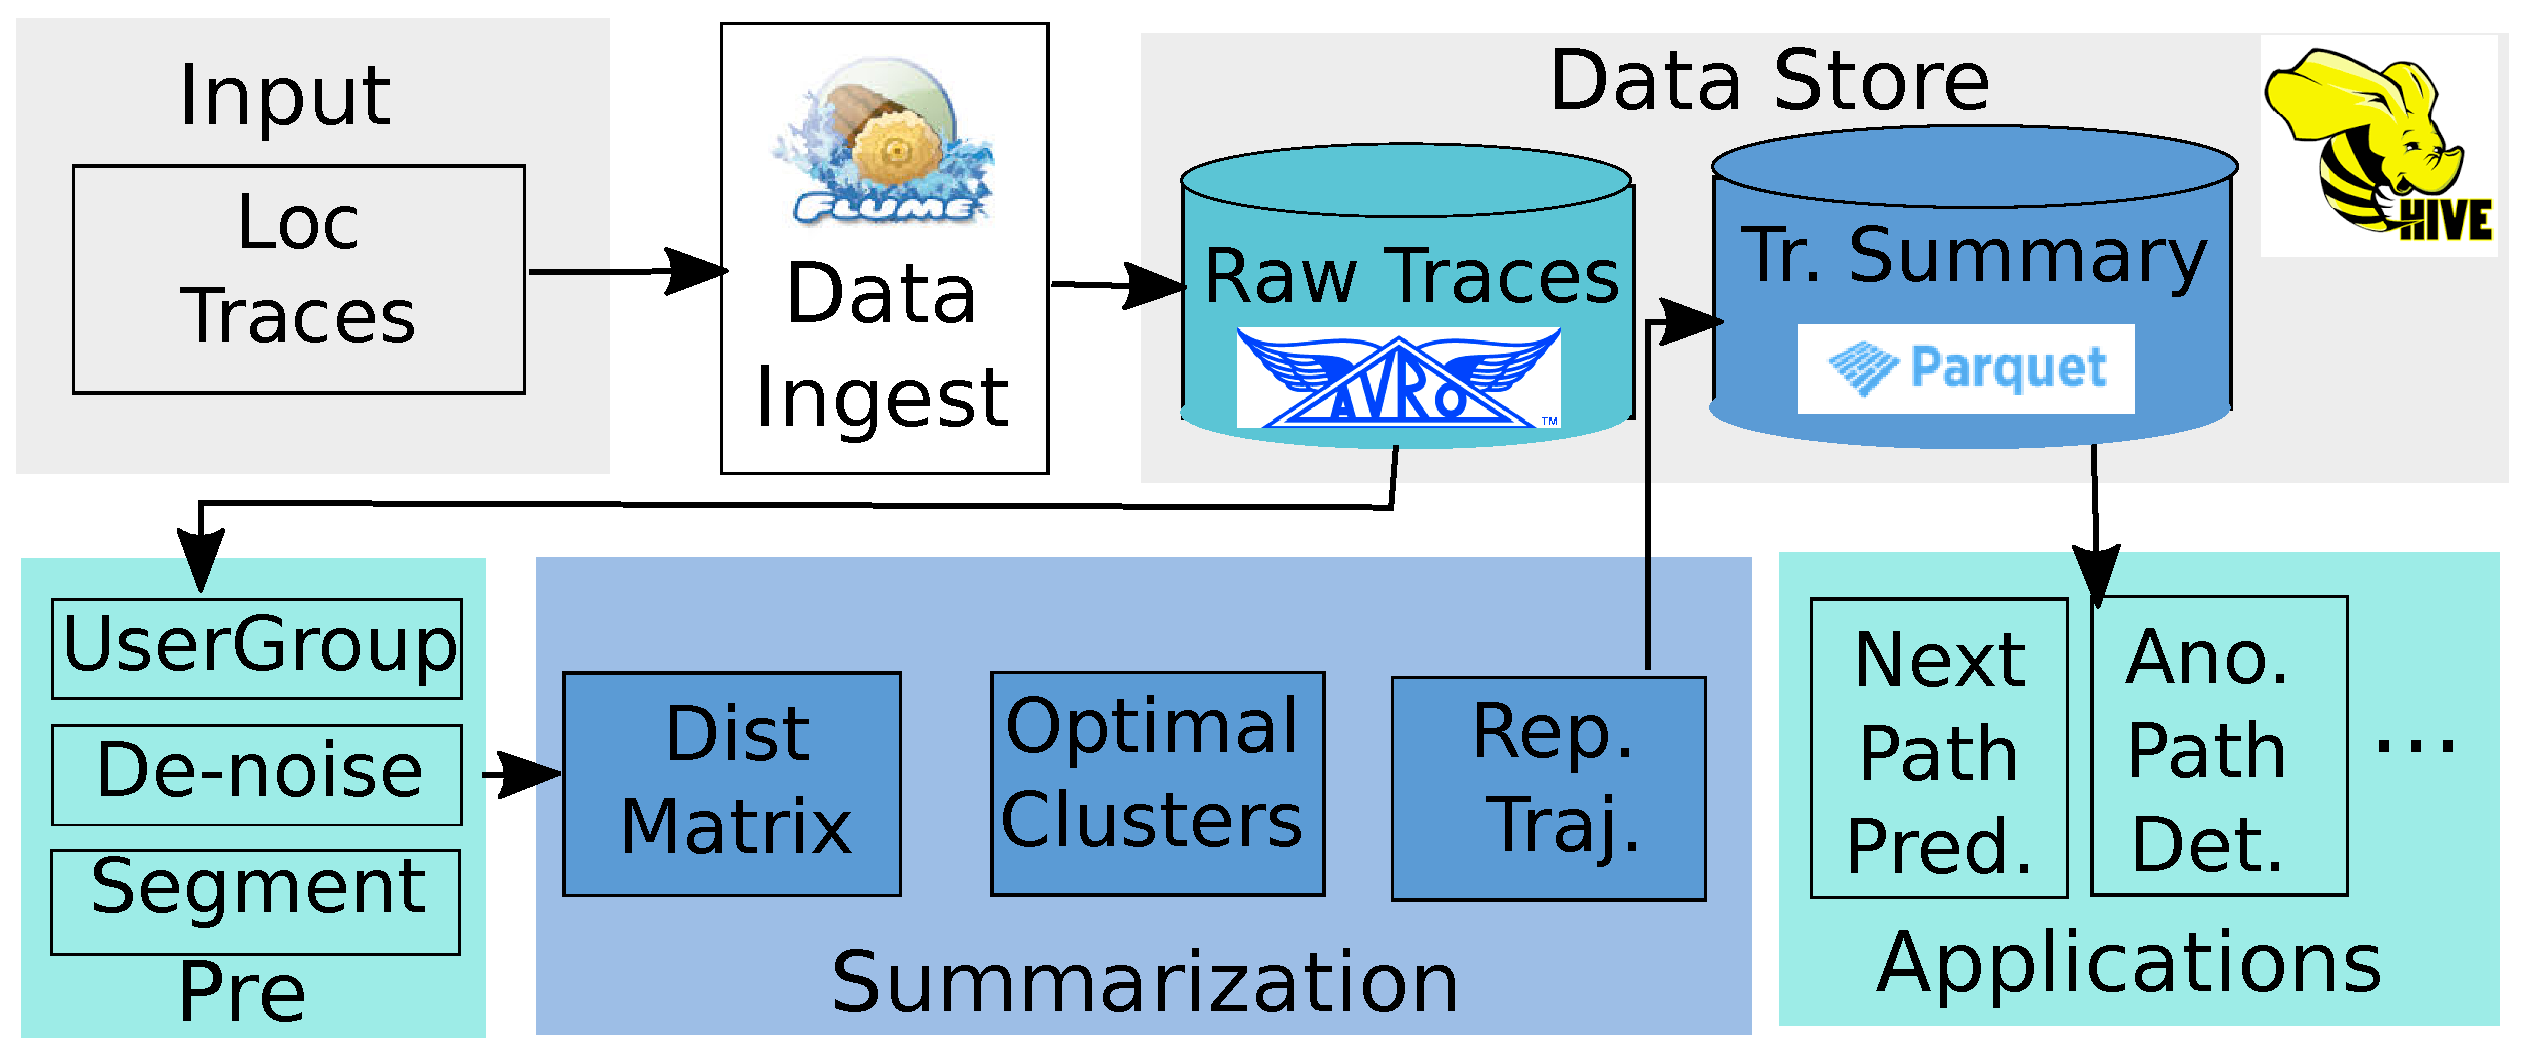
\includegraphics[scale=0.15]{figs/arch1.eps}
\caption{Conceptual Architecture}
\label{fig:flow}
\end{figure}

\begin{figure*}
    \centering   
		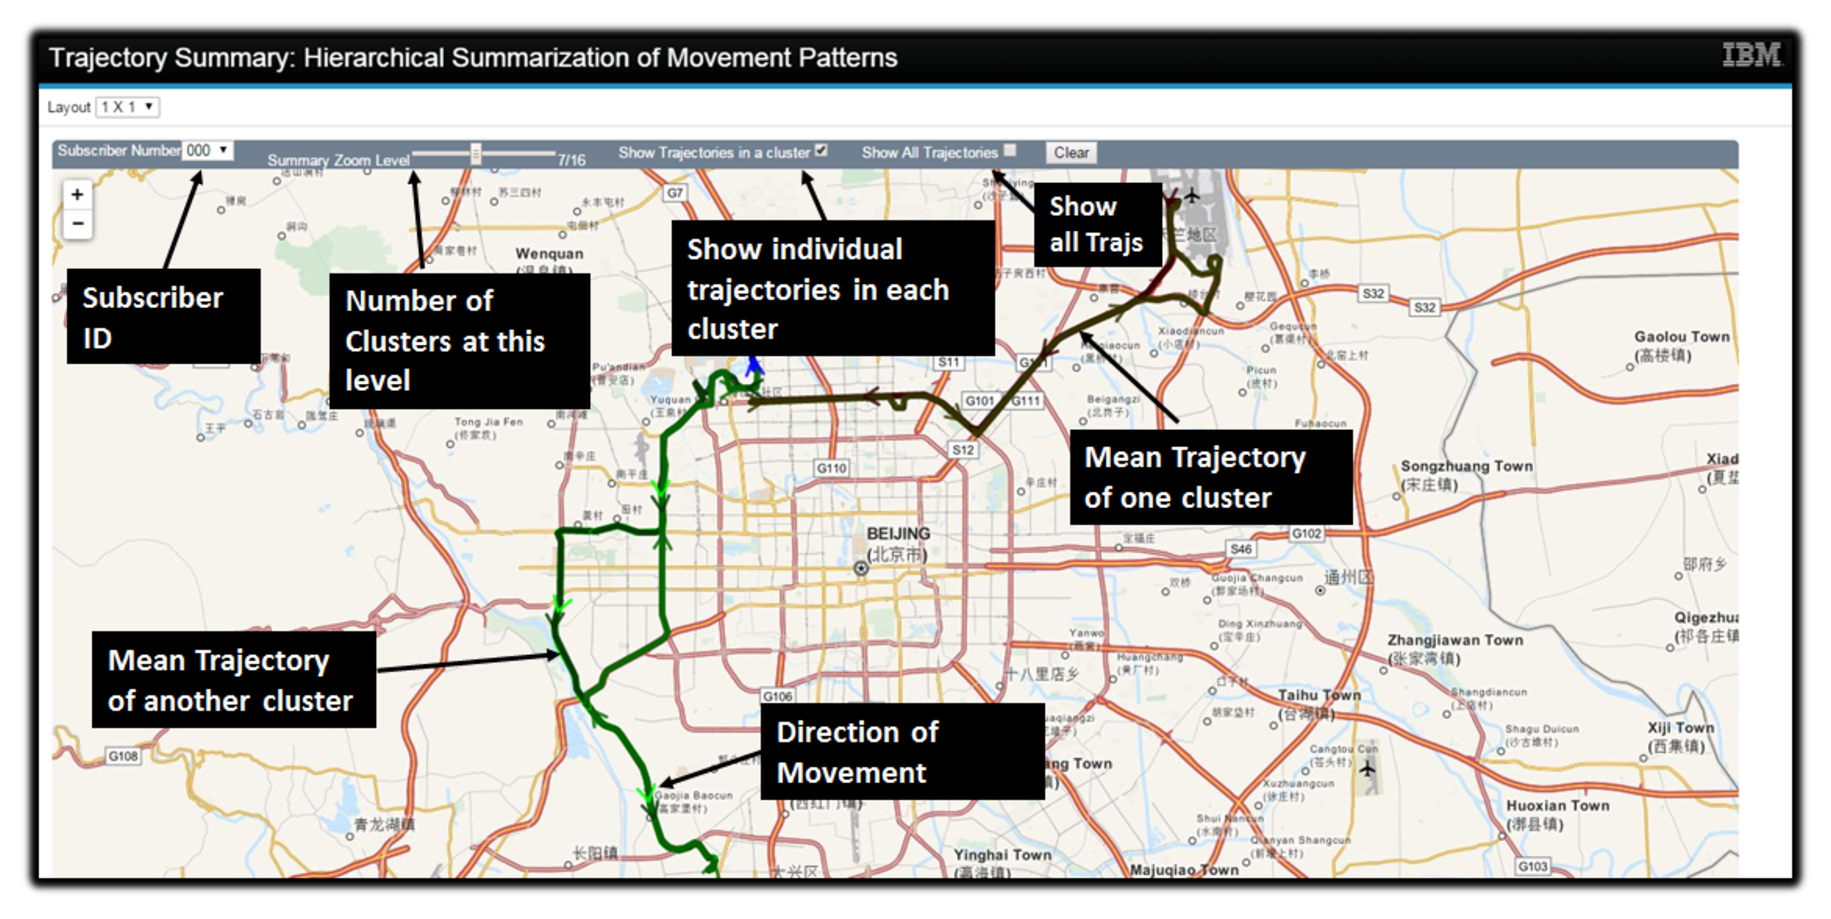
\includegraphics[scale=0.5]{figs/visual.eps}
		\caption{Visualization Framework.}
		\label{fig:vis}  
\end{figure*}

We have developed \trajSummary on Hadoop-based framework for processing large-scale movement summaries. Fig \ref{fig:flow} describes the conceptual architecture. 

\paragraph{Data Ingestion} 
The input to the system is a continuous stream of raw location traces of different users. Each location trace record at-least consists of user identifier, spatial coordinates (latitude and longitude) and time of sample. We use Apache Flume~\cite{flume} to load the real-time traces being continuously deposited in a pre-configured landing directory. The Flume sink then writes the records on the HDFS file system in AVRO format. This data will be mapped as an external table, which is accessible to our analytics modules implemented in Apache Hive~\cite{hive}. Note that the data ingestion happens in real-time; Flume converts and stores the AVRO location samples as and when the location samples arrive in our landing directory

\paragraph{Pre-processing}
\label{sec:preprocess}
Pre-processing stage and the later steps are currently implemented as Batch Analytics. Batch Analytics is executed periodically, which aggregates the records in the past period, and creates data that can be used by the analytics.

In the pre-processing stage, we perform three main tasks: User Grouping, De-noising and Trajectory Segmentation. User Grouping groups location samples of all users into a Hive table in Parquet format. Parquet format is adopted since it provides columnar compression which is useful for our data-sets. This step is necessary since the data is flowing into the system from multiple users at the same time, and our analytics input is the location traces (trajectories) of individual users.

De-noising module filters the outlier GPS traces. We use existing outlier detection algorithms to prune the raw locations~\cite{Yuan2013,Zheng2009}. Such techniques estimate the speed between the consecutive sample points of a user, and prune the points if the speed is greater than a certain threshold (\unit{300}{kmph} in our case).

Trajectory Segmentation identifies the meaningful trips of a user from raw location traces. It utilizes well-known stay-point estimation approaches~\cite{trajcut3}, and stores the \textit{User Trajectories} table. Each trip is stored as an ordered set of 3-tuples $\langle \operatorname{latitude},\operatorname{longitude}, \operatorname{time} \rangle$.

\paragraph{Summarization}
Summarization module is the main contribution of the paper. It inputs the data from the \textit{User Trajectories} table, and stores the user-summaries into the \textit{Traj. Summary} table. We propose and evaluate techniques to compute the summaries for a set of user-trajectories. We show that optimal movement summaries requires understanding of three fundamental concepts: (1) Defining the distance metric between two user trips (Section~\ref{sec:trajDist}); (2) Finding the optimal cluster of user trips that represents a trajectory summary (Section~\ref{sec:trajCluster}); and (3) Representing summaries using a representative trajectories, which can be utilized by the downstream applications (Section~\ref{sec:repTraj}). 

\paragraph{Applications}
The summarization module provides a compact abstraction for applications that query ``frequent-mobility''. Several use-cases can utilize the summary representation of the mobility pattern to provide insights. Next-path prediction problem and Anomalous Movement Detection are example applications that benefit from \trajSummary.

\paragraph{Visualization}
\label{sec:vis}
Fig. \ref{fig:vis} shows a screen-shot of the visualization framework which has been created to work with the trajectories, and the summaries of the user. The interactive framework shows the mobility summary different users. The tool allows exploration of clusters formed at various zoom levels of space. With this flexibility, the tool allows choosing arbitrary level of abstraction of movement summary (e.g., at a city level or at a more granular trajectory level). 
%Once the number of clusters( say k) is set, the k clusters formed will be shown, each cluster in a different colour. 
The tool shows the representative trajectory of each cluster; the thickness is proportional to the number of trajectories in the cluster. Further, each cluster can be individually chosen and inspected. 

\begin{comment}
Various trajectory similarity metrics, which give an estimate of the trajectory distance, have been proposed. Standard LP-Norm and ERP have been shown to be metrics~\cite{Chen2004}, where as other heuristic functions (such as LCSS, DTW, EDR) are non-metrics~\cite{Vlachos2002,Yi1998,Chen2005}. We enhance LP-Norm to construct ``Weighted LP-Norm"', where more weights are given to the points closer to the origin and destination. This is based on the observation that, generally, a user's meaningful trip has an associated intention of commuting between two end-points (such as commuting to work or grocery shop visit).

\noindent\textbf{3. Trajectory Clustering}: 
In this module, hierarchical clustering is applied on the previously computed distance matrix. We choose hierarchical clustering because it gives us a way to store the trajectories of the user at various levels of granularity. Hierarchical clustering involves the computation of a dendrogram which describes how the trajectories are clustered throughout the various levels. We devise a function to cut the dendogram to form the right clusters based on earth-distance between the trajectory points of a cluster.
%The major obstacle is in finding the right number of clusters('k'). The most widely used method in literature to find the value of 'k' is to draw the plot of the number of clusters vs. Sum of Squared Errors within clusters, and finding the elbow point in the plot. However, in the case of human mobility, the clusters formed at the elbow point are very noisy. The heuristic we apply to come up with tighter, meaningful clusters is to go down the dendrogram, starting from the elbow point and reporting final clusters as and when the maximum point-wise earth-distance between all two trajectory pairs is less than a specified threshold $\delta$.

\noindent\textbf{4. Representative Trajectory:} 
We summarize the significant clusters by a representative trajectory for that cluster. We utilize the median trajectories~\cite{median1} because it provides parts of actual user traveled paths as representative trajectory.\\
\end{comment}